\chapter{Introduction}
\label{chap:intro}

The major goal of this line of research is to develop
high order, numerically stable fast algorithms for solving elliptic
partial differential equations using the Minimum Sobolev norm (MSN).
This will require much more work than can be completed in one dissertation.
The present work focuses on developing fast algorithms to solve interpolation
and ordinary differential equation problems using the MSN method,
which will be a stepping stone to understand the
structure of the matrices arising in 2D and 3D PDEs.
We introduce these ideas by discussing some of the problems
present in interpolation methods and how the MSN method
attempts to solve them.



\section{Lagrange Interpolation and Known Difficulties}
\label{sec:int_class_interp}

The well-known Weierstrass Approximation Theorem, which we reproduce for
completeness, says continuous functions on compact, connected intervals can
be approximated arbitrarily well by polynomials:

\begin{thm}[Weierstrass Approximation Theorem;
    Theorem 7.26 in \cite{baby_rudin}]
\label{thm:WeierstrassThm}
If $f\in C[a,b]$, then there exists a sequence
of polynomials $\braces{P_{n}}_{n=1}^{\infty}$ such that

\begin{equation}
    \lim_{n\to\infty} \norm{f-P_{n}}_{\infty,[a,b]} = 0.
\end{equation}
\end{thm}

\noindent
Here,

\begin{equation}
    \norm{g}_{\infty,[a,b]} \equiv \sup_{x\in\brackets{a,b}} \abs{g(x)}
\end{equation}

\noindent
is the supremum norm.
When the interval $\brackets{a,b}$ is understood, we may
write $\norm{\cdot}_{\infty}$ in place of $\norm{\cdot}_{\infty,[a,b]}$.
This theorem shows that the set of polynomials $\mathcal{P}$
is dense in $C[a,b]$, the space of continuous functions on $[a,b]$.
We let $\mathcal{P}_{n}$ denote all polynomials of degree at most $n$.
This gives rise to an important concept: degree of
approximation.
We also have the following theorem:

\clearpage

\begin{thm}[Best Uniform Approximation of Continuous Functions;
    Section 1.1 in~\cite{rivlin2003introduction}]
If $f\in C[a,b]$ and $n\in\N_{0}$, then there exists
a unique $q_{n}\in\mathcal{P}_{n}$ so that
%
\begin{equation}
    \norm{f-q_{n}}_{\infty} = \inf_{p\in\mathcal{P}_{n}}\norm{f-p}_{\infty}.
\end{equation}
%
We set
%
\begin{equation}
    E_{n}(f) \equiv \inf_{p\in\mathcal{P}_{n}}\norm{f-p}_{\infty}
\end{equation}
%
and have
%
\begin{equation}
    E_{0}(f)\ge E_{1}(f)\ge E_{2}(f) \ge \cdots \to 0.
\end{equation}
\end{thm}

There are many ways to prove the Weierstrass Approximation theorem.
In~\cite[Chapter 7]{baby_rudin}, Rudin convolves against a polynomial kernel.
This is useful theoretically but in practice, one may only
have function and derivative information at particular points.
In order to reconstruct the underlying function, we want to use
these function and derivative values to build an approximation,
frequently chosen to be a polynomial.
This is interpolation.

\textbf{Interpolation Problem:} Let $f\in C[-1,1]$ be continuous
and specify a sequence of grid points

\begin{equation}
    -1\le x_{1;n} < x_{2;n} < \cdots < x_{n;n}\le1.
\end{equation}

\noindent
for $n\in\N$.
Determine a polynomial $p_{n}$ with $\deg p_{n} = m(n)$
which satisfies the conditions

\begin{equation}
    f(x_{k;n}) = p_{n}(x_{k;n}),
\end{equation}

\noindent
and ascertain under what restrictions on $f$ and $\braces{x_{k;n}}_{k=1}^{n}$
ensure

\begin{equation}
    \norm{f-p_{n}}_{\infty} \to0,\quad n\to\infty.
\end{equation}

A popular choice is to set $m(n) = n-1$, resulting in Lagrange
interpolation.
In Fig.~\ref{fig:intro_runge_plot}, we see an example of Lagrange
interpolation on equally-spaced nodes of the Runge function
$\brackets{1+25x^{2}}^{-1}$ on $[-1,1]$.
This function is analytic; even so, in~\cite{runge1901} Runge
proved that Lagrange interpolation diverges in this case.
In particular, there are large oscillations near the boundary points.

% Plot of Runge phenomenon
% Runge figure
\begin{figure}[t]
\centering
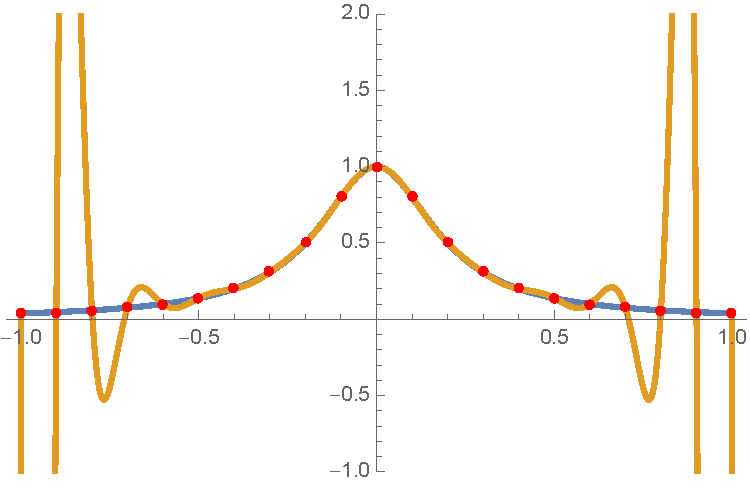
\includegraphics[width=10cm]{plots/runge_phenomenon.pdf}
\caption[Example of the Runge phenomenon]{
Here is an example of Lagrange interpolation of the Runge function
$\brackets{1+25x^{2}}^{-1}$ using Lagrange interpolation
with 21 equally-spaced nodes.}
\label{fig:intro_runge_plot}
\end{figure}


In fact, much more is known about Lagrange interpolation,
and we introduce notation which will make this discussion easier.
Let

\begin{equation}
    X = \braces{x_{k;n} \mid k=1,\cdots,n; n\in\N}
\end{equation}

\noindent
be an interpolatory matrix. Then, given $f\in C[-1,1]$,
we have the following standard
definitions~\cite[Chapter 1]{interpFunctionsBook}:

\begin{samepage}
\begin{align}
    L_{n}(f,X,x) &= \sum_{k=1}^{n}\ell_{k,n}(X,x)f(x_{k;n}) \nonumber\\
    \Omega_{n}(X,x) &= \prod_{i=1}^{n}\parens{x-x_{i;n}}
        \nonumber\\
    \ell_{k,n}(X,x) &= \frac{\Omega_{n}(X,x)}{\Omega_{n}'(X,x_{k;n})(x-x_{k;n})}
        \nonumber\\
    \lambda_{n}(X,x) &= \sum_{k=1}^{n}\abs{\ell_{k,n}(X,x)} \nonumber\\
    \Lambda_{n}(X) &= \norm{\lambda_{n}(X,x)}_{\infty,[-1,1]}.
\end{align}
\end{samepage}

\noindent
Naturally, $L_{n}(f,X,x)$ is the Lagrange interpolating polynomial
of degree at most $n-1$ for the interpolation matrix $X$.
The Lebesgue constants $\Lambda_{n}(X)$ are of
critical importance, as we see

\begin{align}
    \abs{L_{n}(f,X,x) - f(x)} &\le \abs{L_{n}(f,X,x) - q_{n-1}(x)}
            + \abs{f(x) - q_{n-1}(x)} \nonumber\\
    &\le \abs{L_{n}(f-q_{n-1},X,x)} + E_{n-1}(f) \nonumber\\
    &\le \brackets{\Lambda_{n}(X)+1}E_{n-1}(f).
    \label{eq:Ln_upper_bound_err}
\end{align}

\noindent
Here, $q_{n-1}\in\mathcal{P}_{n-1}$ is the minimizer in the supremum norm,
and we note $L_{n}:\mathcal{P}_{n-1}\to\mathcal{P}_{n-1}$ is the identity map.
Because $E_{n}(f)\to0$, Lagrange interpolation converges when
$\Lambda_{n}(X)E_{n-1}(f)\to0$.

If we could find an interpolatory matrix $Y$ so that $\Lambda_{n}(Y)$ is
bounded, then $L_{n}(f,Y)\to f$ uniformly. Unfortunately, this is not
the case. In~\cite{vertesi1990optimal}, V\'{e}rtesi references Faber (1914)
as proving

\begin{equation}
    \Lambda_{n}(X) > \frac{1}{8\sqrt{\pi}}\log n
\end{equation}

\noindent
for every $X$, showing $\Lambda_{n}(X)$ is unbounded.
One popular set of interpolation nodes is the zeros
of the Chebyshev polynomials:

\begin{align}
    T &= \braces{z_{k}^{n} \mid k=1,\cdots,n; n\in\N} \nonumber\\
    z_{k}^{n} &= \cos\brackets{\frac{\pi}{n}\parens{n-k+\frac{1}{2}}}.
\end{align}

\noindent
The Chebyshev polynomials $T_{n}(x)$ are a set of orthogonal polynomials
which will be discussed in detail in Sec.~\ref{ssec:kar_cheby}.
In~\cite{Brutman1978}, it was shown

\begin{equation}
    \Lambda_{n}(T) < 8 + \frac{2}{\pi}\log n,
\end{equation}

\noindent
For this reason, we see that the interpolatory matrix $T$
is close to optimal and,
coupled with fast interpolation methods, gives reason
for its popularity. Better bounds for Lebesgue
constants can be found in~\cite{smith2006lebesgue}.

We also give bounds for equally-spaced points, setting

\begin{equation}
    E = \braces{\left. -1+2\frac{k-1}{n-1} \right| k=1,\cdots,n; n\in\N}.
\end{equation}

\noindent
In~\cite{trefethen1991two}, Trefethen and Weideman give the bounds

\begin{equation}
    \frac{2^{n-2}}{n^{2}} < \Lambda_{n}(E) < \frac{2^{n+3}}{n}
\end{equation}

\noindent
as well as referencing the asymptotic result and some of the history
of equally-spaced interpolation.
Clearly, the exponential growth of
$\Lambda_{n}(E)$ helps quantify how much worse $E$ is when
compared with $T$.

This divergence is not restricted to equally-spaced point
distributions, though.
In fact, we have the following result:

\begin{thm}[Theorem 4.3 in~\cite{interpFunctionsBook}]
For an interpolatory matrix $X\subset[-1,1]$, there exists $h\in C[-1,1]$
so that
%
\begin{equation}
    \limsup_{n\to\infty} \abs{L_{n}(h,X,x)} = \infty
\end{equation}
%
for almost every $x\in[-1,1]$.
\end{thm}

\noindent
So, there is no interpolatory matrix $Y$ so that
$\norm{L_{n}(f,Y)-f}_{\infty}\to0$ for all continuous functions $f$
and the approximation error can be arbitrarily bad.



\section{Possible Solutions to Divergence of Lagrange Interpolation}
\label{sec:poss_lagrange_sol}

Although the previous result paints a bleak picture of Lagrange interpolation,
this is true only in extreme situations.
From~\cite[Chapter 1]{rivlin2003introduction}, we have the following theorem
discussing how the degree of approximation is related to smoothness:

\begin{thm}[Jackson Inequality]
\label{thm:best_uni_err}
If $g\in C^{k}[-1,1]$ and $g^{(k)}$ is $\alpha$-H\"{o}lder
with H\"{o}lder constant $L$, then for $n>k$, we have
%
\begin{equation}
    E_{n}(g) \le \frac{c}{n^{k}}\parens{\frac{1}{n-k}}^{\alpha}
\end{equation}
%
with $c=6^{k+1}e^{k}(1+k)^{-1}L$.
\end{thm}

\noindent This theorem shows that if $g$ is merely $\alpha$-H\"{o}lder
continuous, then $\norm{L_{n}(g,T)-g}_{\infty}\to0$ by
Eq.~\eqref{eq:Ln_upper_bound_err}.
As noted above, we can have $\norm{L_{n}(f,E)-f}_{\infty}\not\to0$
even when $f$ is analytic.

We previously noted $L_{n}(f,E)$ has large oscillations in the Runge example.
Because of this, there has been interest in Hermite-Fej\'{e}r interpolation.
Given an interpolatory matrix $X$, we let $H_{n}(f,X,x)\in\mathcal{P}_{2n-1}$
so that

\begin{align}
    H_{n}(f,X,x_{k;n}) &= f(x_{k;n}) \nonumber\\
    H_{n}'(f,X,x_{k;n}) &= 0.
\end{align}

\noindent
In this case, it can be shown $\norm{H_{n}(f,T)-f}_{\infty}\to0$
as $n\to\infty$ for all $f\in C[-1,1]$~\cite[Chapter 5]{interpFunctionsBook}.
Unfortunately, this does not hold in general; in fact,
for equally-spaced nodes we have the particularly bad
result

\begin{align}
    f(x) &= x \nonumber\\
    \limsup_{n\to\infty} \abs{H_{n}(f,E,x)} &= \infty,\quad 0 <\abs{x}\le1,
\end{align}

\noindent
which is discussed in~\cite[Chapter 6]{interpFunctionsBook}.
Controlling the derivative of the interpolation polynomial
at the Chebyshev nodes appears to give sufficient control of the polynomial
in order to obtain convergence for all continuous functions.
Even so, while this gives convergence in the limit,
it is not useful in practice because we purposefully limit the
accuracy of interpolation near, but not at, interpolation nodes.

In another direction, Bernstein polynomials give up interpolation
to get overall approximation.
In fact, \cite{davis_interpolation,rivlin2003introduction}
use Bernstein polynomials to prove the Weierstrass Approximation Theorem.
The downside is that convergence to the solution is slow:

\clearpage

\begin{thm}[Error Estimate for Berstein polynomials;
    Theorem 1.2 in \cite{rivlin2003introduction}]
\label{thm:berstein_polynomial_error}
Suppose $g\in C[0,1]$ is $\alpha$-H\"{o}lder
with H\"{o}lder constant $L$ and $B_{n}g$ is the Berstein
polynomial of degree $n$ for $g$; then 
%
\begin{equation}
    \norm{g - B_{n}g}_{\infty,[0,1]} \le
        \frac{3L}{2}\frac{1}{n^{\alpha/2}},
\end{equation}
%
and this bound in $n$ cannot be improved.
\end{thm}

\noindent
This precludes it from being of much use in practice,
especially when $f$ is smooth.

By relaxing the condition $\deg L_{n}(f,X) \le n-1$,
Erd\H{o}s was able to prove in~\cite{erdos1943some} that,
under some conditions on $X$, one could prove convergence
for all continuous functions by choosing $p_{n}$ so that
$\deg p_{n} = c(X)n$, with $c$ a constant depending only on $X$.
The extension to all matrices $X$ is shown
in~\cite[Theorem 2.7]{interpFunctionsBook}.
This is important in practice, because we can not
always choose the interpolation nodes.
It is beneficial for a method to work well independent of
node location, especially if, because of instrument specifications,
data collection location cannot be modified.
Unfortunately, these results require function values at arbitrary points,
and this is not possible in practice.



\section{Interpolation in Higher Dimensions}
\label{sec:Interp_MD}

Up to this point, we have only talked about methods for approximating
functions on $[a,b]$; even so, many problems in science and engineering
are inherently two- and three-dimensional.
A review of recent methods for multivariable polynomial interpolation
can be found in~\cite{gasca2001history,gasca2000polynomial}.
One challenge of interpolation in higher dimensions is choosing 
the correct polynomial space and point distribution.
Now, the fact $\dim \mathcal{P}_{n-1}=n$ makes this easy in 1D
but in higher dimensions there does not appear to be a simple way to
choose a multivariable polynomial space of arbitrary dimension.
Naturally, this is a topic of great interest.
In~\cite{gasca2000polynomial}, some standard methods discussed include
tensor products of univariate polynomials, Gr\"{o}bner bases,
and ideal interpolation schemes.



\section{Hermite and Birkhoff Interpolation}
\label{sec:Birkhoff_MD}

Hermite or Birkhoff interpolation problems involve interpolating
function and derivative values.
Hermite interpolation consists of interpolating function and derivative
values up to a certain degree at interpolation nodes.
Birkhoff interpolation is more general, allowing any combination
of specified function and derivative values at nodes.
Hermite interpolation is well-posed and can easily be solved in 1D.
This is not the case for Birkhoff interpolation, where only
certain combinations ensure a unique
solution~\cite{karlin1972hermite,lorentz1971birkhoff}.
The problem is even more complicated in dimension 2 and larger;
see~\cite{lorentz2000multivariate,rudy} for a review of these topics.
An additional challenge in multidimensional interpolation
comes from proving error bounds and determining sufficient conditions for
convergence.



\section{Characteristics of Good Algorithms}
\label{sec:Good_Alg_Details}

This dissertation focuses on the development, implementation,
and analysis of fast MSN methods. The ideas behind the MSN method
will be discussed in the Sec.~\ref{sec:msn_intro}, but here
we discuss good qualities that numerical algorithms should have,
especially algorithms for approximation.
These are high-order convergence, low computational complexity,
and numerical stability.

Given a low-order method and a high-order method of similar computational cost,
a faster-converging method is more effective and useful.
In practice, there is always a limit to the amount of computational
resources (memory, processor speed, or bandwidth), so a high-order
method would be preferred as it would lead to less work overall.
As mentioned before, Bernstein polynomials converge to all
continuous function but do so at a slow rate. This alone does not
necessarily disqualify the algorithm, but from Thm.~\ref{thm:best_uni_err},
we know smoother functions can have better polynomial
approximations. This incentivizes developing accurate approximations
and algorithms to compute them.

While some methods may be of theoretical importance, algorithms will only
be of practical value if there are efficient methods to compute them.
The total cost should be of reasonable size, so that both the 
asymptotic growth ($O(\log n)$ or $O(n^{3})$) and
the explicit cost ($10^{6}\log n$ and $\frac{2}{3}n^{3}$) are important.
Because computational resources are always limited, asymptotics
may not be as important as the prefactor hidden by Big O notation.

Finally, numerical stability is of critical importance.
Almost all algorithms are implemented on computers using
floating-point arithmetic, inevitably leading to small errors.
It is necessary for practical algorithms to be immune to these
changes; namely, small changes in inputs should lead to small changes
in outputs.
The condition number quantifies how much changes in outputs come
from changes in inputs; a standard reference for numerical stability
is~\cite{HighamASNA}.



\section{The Minimum Sobolev Norm Method}
\label{sec:msn_intro}

We previously showed Lagrange interpolation
does not work, for there can be large oscillations in the interpolating
polynomial as seen in the Runge phenomenon, while using a polynomial
of higher degree allows continuous functions to be approximated
arbitrarily well.
By combining these observations, the 
Minimum Sobolev norm (MSN) method was developed: a general
method for computing approximate solutions to problems
with linear constraints.

The MSN method has been used to solve problems in
interpolation~\cite{msnInterp},
Birkhoff interpolation~\cite{msnBirkhoff}, and
partial differential equations~\cite{msnPDE},
For simplicity,
we assume we are performing approximations using algebraic polynomials,
even though theoretical work often uses trigonometric polynomials.
The main idea is this: given $N$ linear constraints and polynomials
of up to degree $M(N)$ contained in $V$, unknown coefficients $a$,
correct values $f$, and a diagonal matrix $D_{s}$ with
condition number $O(M^{s})$, the MSN solution solves the equation

\begin{equation}
    \min_{Va=f} \norm{D_{s}a}_{2}.
    \label{eq:msn_def}
\end{equation}

\noindent
We choose $D_{s}$ so that $\norm{D_{s}a}_{2}$ is a Sobolev norm.
This implies that we seek an approximation which satisfies the linear
constraints as well as having the smallest derivative norm.
Here we focus on computing the minimum 2-norm solution
because this dissertation investigates efficient numerical algorithms
for MSN equations and we explicitly compute LQ factorizations;
methods for $p$-norm minimization are discussed in~\cite{msnInterp,msnBirkhoff}.
Additionally, this description is independent of dimension and node location.
The parameter $s$ determines which derivative of the
polynomial approximation we wish to control.
Larger $s$ gives more derivative control on the approximation
but leads Eq.~\eqref{eq:msn_def} to have higher condition
numbers. Great care is required to limit the effects of these
condition numbers in order to ensure convergence to the underlying
solution~\cite{msnBirkhoff}.

The technical challenge of this method is to determine
the explicit form of $M(N)$ to ensure convergence to the solution.
The methods in~\cite{msnInterp,msnBirkhoff} involve the close
approximation of integral kernels by polynomials.
The end result is that it is sufficient to choose $M(N) = C\eta^{-1}$,
where $\eta$ is the minimum separation between between
interpolation nodes. Although this is a theoretically optimal result,
knowing from~\cite{interpFunctionsBook} that this result cannot
be improved except in the constant, it is not useful in practice
because the constants from~\cite{msnInterp,msnBirkhoff}
are difficult to explicitly compute.
In practice, we have found that choosing the $M(N) = 2\pi\eta^{-d}$
is sufficient, where $d$ is the dimension of the space.
These details, along with
implementation issues, will be discussed more in the next section.

One advantage of the MSN method is that we do not insist on forming
a square linear system.
In fact, it is necessary
to take enough columns (more than twice the number of rows)
in order to ensure a good approximation. Choosing the proper
polynomial space was a challenge mentioned in Secs.~\ref{sec:Interp_MD}
and \ref{sec:Birkhoff_MD}.



\section{MSN Interpolation Examples}
\label{sec:MSN_slow_examples}

We present some results of MSN interpolation on equally-spaced
nodes in single and double precision for 1D and 2D.
We do this to show that the difficulty of approximating
functions on equally-spaced points arises from using suboptimal methods
of interpolation rather than node location.
These and similar results were published in~\cite{msnInterp,msnBirkhoff}.

We can rewrite Eq.~\eqref{eq:msn_def} as

\begin{align}
    &\min_{VD_{s}^{-1}x=f} \norm{x}_{2} \nonumber\\
    &\quad a = D_{s}^{-1}x.
    \label{eq:msn_def_rework}
\end{align}

\noindent
In order to compute the MSN solution,
we must compute the minimum norm solution from Eq.~\eqref{eq:msn_def_rework}.
To do this, we must compute an LQ factorization of $VD_{s}^{-1}$,
where $L$ is a lower triangular matrix and $Q$ is orthogonal.
As previously mentioned, large $s$ leads to greater derivative control
but also gives $VD_{s}^{-1}$ high condition number. Because
of this, the standard pivoted LQ factorization based on QR with
Column Pivoting is insufficient. A Rank-Revealing QR factorization
based on~\cite{gu1996efficient} would be better, but an 
implementation is not readily available so we use another method presented
here and described in~\cite{msnBirkhoff}; see Alg.~\ref{alg:slow_msn_lq}.

\begin{algorithm}[t]
\caption{Slow, stable algorithm for solving MSN systems}
\label{alg:slow_msn_lq}
\begin{algorithmic}[1]
\Function{slow\_msn\_solve}{$f$,$V$,$D_{s}$}
\Comment{Solve $\min_{Va=f}\norm{D_{s}a}_{2}$.}
    \State Compute $P_{1}L_{1}Q_{1}=V$ using an LQ factorization
        based on QRCP.
    \State Determine permutation $\Pi$ such that $Q_{1}D_{s}^{-1}\Pi$
        has decreasing column norms.
    \State Compute the SVD:
        $U\Sigma V^{*} = Q_{1}D_{s}^{-1}\Pi$; only $U$ is stored.
    \State Compute $P_{2}L_{2}Q_{2} = U^{*}Q_{1}D_{s}^{-1}\Pi$.
    \State Solve $L_{1}z = P_{1}^{*}f$.
    \State Solve $L_{2}y = P_{2}^{*}U^{*}z$.
    \State Set $a = D_{s}^{-1}\Pi Q_{2}^{*}y$
    \State \Return $a$
\EndFunction
\end{algorithmic}
\end{algorithm}


The unique feature of the algorithm may be Lines 4 and 5.
Clearly, $VD_{s}^{-1}$ is badly column-scaled.
LQ factorizations can deal with poor row-scaling but not poor column-scaling.
We compute the singular value decomposition
$U\Sigma V^{*} = Q_{1}D_{s}^{-1}\Pi$ in Line 4 and
see $U^{*}Q_{1}D_{s}^{-1}\Pi \approx \Sigma V^{*}$ to machine precision.
This ensures we can accurately compute the pivoted LQ
factorization $P_{2}L_{2}Q_{2} = U^{*}Q_{1}D_{s}^{-1}\Pi$ in Line 5.
Thus, $U$ is a preconditioner for numerical stability, showing
that we can safely convert poor column-scaling to poor row-scaling.
Using Alg.~\ref{alg:slow_msn_lq}, the effective condition number of this
problem appears to be that of $V$ and not $VD_{s}^{-1}$.

Looking at the algorithm, we see two pivoted LQ factorizations
and one SVD are required.
Because we have $N$ interpolation requirements
and $cN$ columns, this gives us $O(N^{3})$ floating-point operations
and $O(N^{2})$ units of memory.
At first glance, this does not seem too bad.
If we are in dimension $d$ with $n^{d}$ tensor grid points, then $N = n^{d}$ and
we require $O(n^{3d})$ flops and $O(n^{2d})$ units of memory.
While these costs may be acceptable for $d=1$ and bearable for $d=2$,
when $d=3$ this is too great.
Parallel computation would not be
of much use here because the communication required for pivoted LQ
and the SVD would cause the entire process to be extremely slow,
although there has been recent work in reducing the communication cost
in pivoted QR factorizations~\cite{demmel2015communication}.
In order for these algorithms to be used when solving large, difficult
problems, we need to investigate other methods.
Similar costs arise when solving differential equations and
this necessitates fast, structured algorithms.
When developing fast algorithms, it is critical
that we are able to convert the poor columns scaling to poor row scaling.
The inherent structure of the linear system allows us to do this
using careful factorizations.

We present some examples of MSN interpolation and Birkhoff interpolation.
The functions we approximate are

\begin{samepage}
\begin{align}
    f(x) &= \frac{1}{1+25x^{2}} \nonumber\\
    g(x,y) &= \frac{1}{1+ 25(x^2 + y - 0.3)^{2}}
       + \frac{1}{1+ 25(x + y - 0.4)^{2}} \nonumber\\
       &\quad + \frac{1}{1+ 25(x + y^{2} - 0.5)^{2}}
       + \frac{1}{1+ 25(x^{2} + y^{2} - 0.25)^{2}}
        \nonumber\\
    h(x) &= g(x,-0.96).
    \label{eq:intro_runge_functions}
\end{align}
\end{samepage}

\noindent
Naturally, $f$ is the usual Runge function. Here, $g$ is a 2D
function with Runge functions on one line, one circle, and two
parabolas.

We remember machine precision is $2^{-23}\approx 1.2\times10^{-7}$ in single
precision and $2^{-52}\approx 2.2\times10^{-16}$ in double precision.
This is the smallest relative error that we could expect for
any nonzero result. All of the plots show results for
$\norm{f-p}_{\infty}/\norm{f}_{\infty}$ for true function $f$
and approximation $p$. The sup-norm is approximated
by sampling the function at a large number of locations and taking
the maximum.

The results for interpolating $f$ are shown in Fig.~\ref{fig:intro_msn_interp}.
For single precision, all error curves decay toward $10^{-7}$ as
we increase the number of points. The main exception is for $s=6$,
which starts to increase around 60 points. We believe this occurs
because of rounding error. This would also make sense given for
$s\in\braces{3,4,5}$, the error curves hover close to $10^{-6}$.
We see a similar results for double precision.
In this case, the beginnings of the U-shaped error curve seem
present for $s\in\braces{8,10,12}$.

In Fig.~\ref{fig:intro_msn_birkhoff_1d}, we have the results
of MSN Birkhoff interpolation in 1D for $h$.
Although the error curve for $s=2$ in single and double precision hovers around
$10^{-3}$, the other error curves decay to machine precision.
The beginning of a U-shaped error curve may be seen
for $s\in\braces{4,5}$ in single precision and $s\in\braces{10,12}$
in double precision. The errors are low, although they may be slightly
larger than those we see in regular MSN interpolation.
This could stem from the fact the condition number is inherently larger for
Birkhoff interpolation than for interpolation.

In Fig.~\ref{fig:intro_msn_birkhoff_2d},
we have results for MSN Birkhoff interpolation in 2D
for $g$ from Eq.~\eqref{eq:intro_runge_functions}.
In every case the error decreases with increasing data except
for $s=5$ with single precision. In this case, we may start
to see the beginning of the effects of roundoff error.
The challenge for 2D problems is the long time required to
run Alg.~\ref{alg:slow_msn_lq}.

\begin{figure}
\centering
    \begin{subfigure}{0.45\textwidth}
    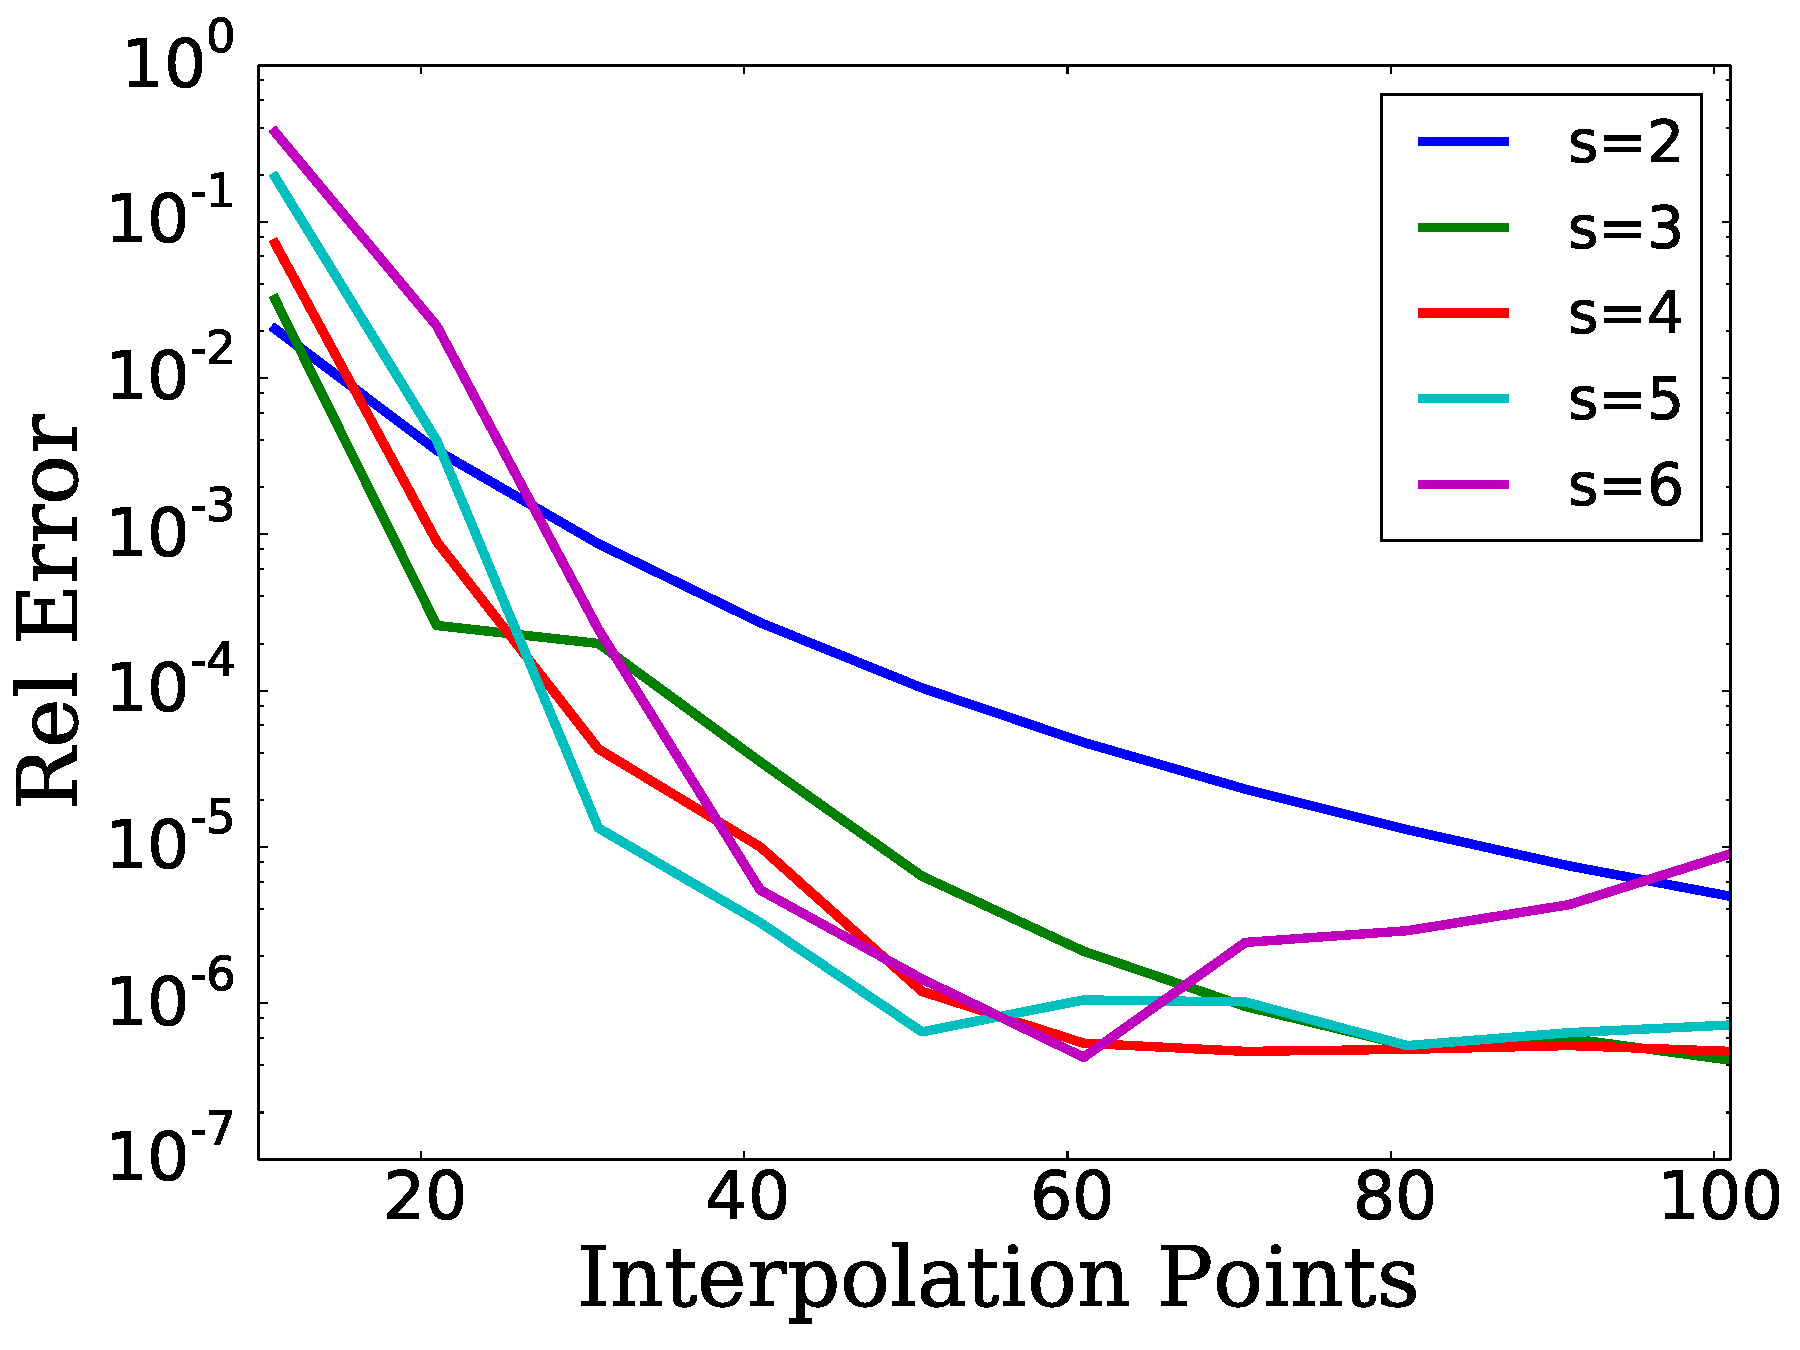
\includegraphics[width=\textwidth]{plots/msn_interp_1d_single_runge.pdf}
    \caption{Single Precision}
    \end{subfigure}
    \begin{subfigure}{0.45\textwidth}
    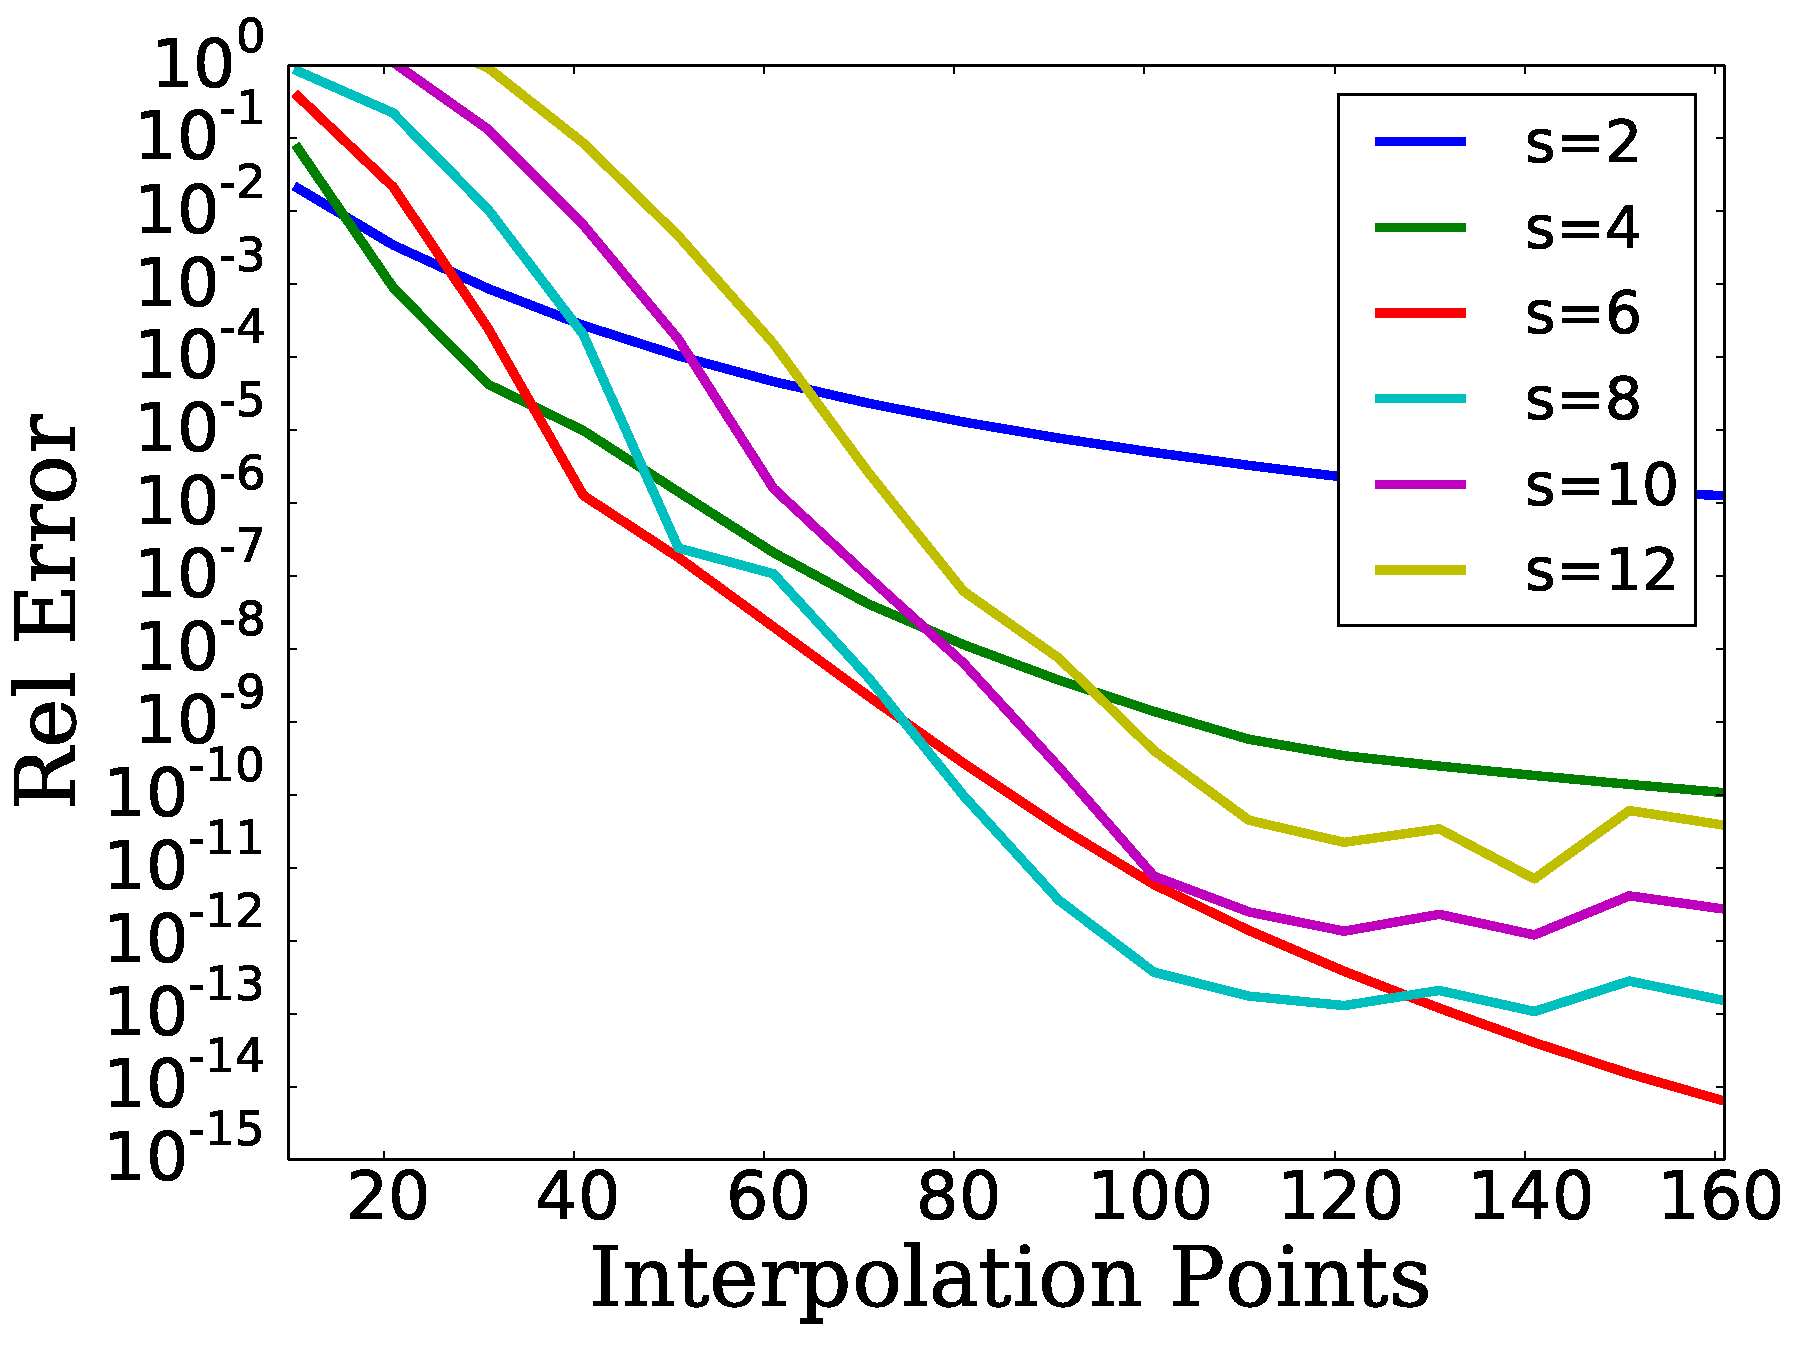
\includegraphics[width=\textwidth]{plots/msn_interp_1d_double_runge.pdf}
    \caption{Double Precision}
    \end{subfigure}
\caption[MSN 1D Interpolation Relative Error]{
Relative error results for MSN interpolation on equally-spaced points
on the function $f(x)$ from Eq.~\eqref{eq:intro_runge_functions}
for various $s$ values using single and double precision.}
\label{fig:intro_msn_interp}
\end{figure}

\begin{figure}
\centering
    \begin{subfigure}{0.45\textwidth}
    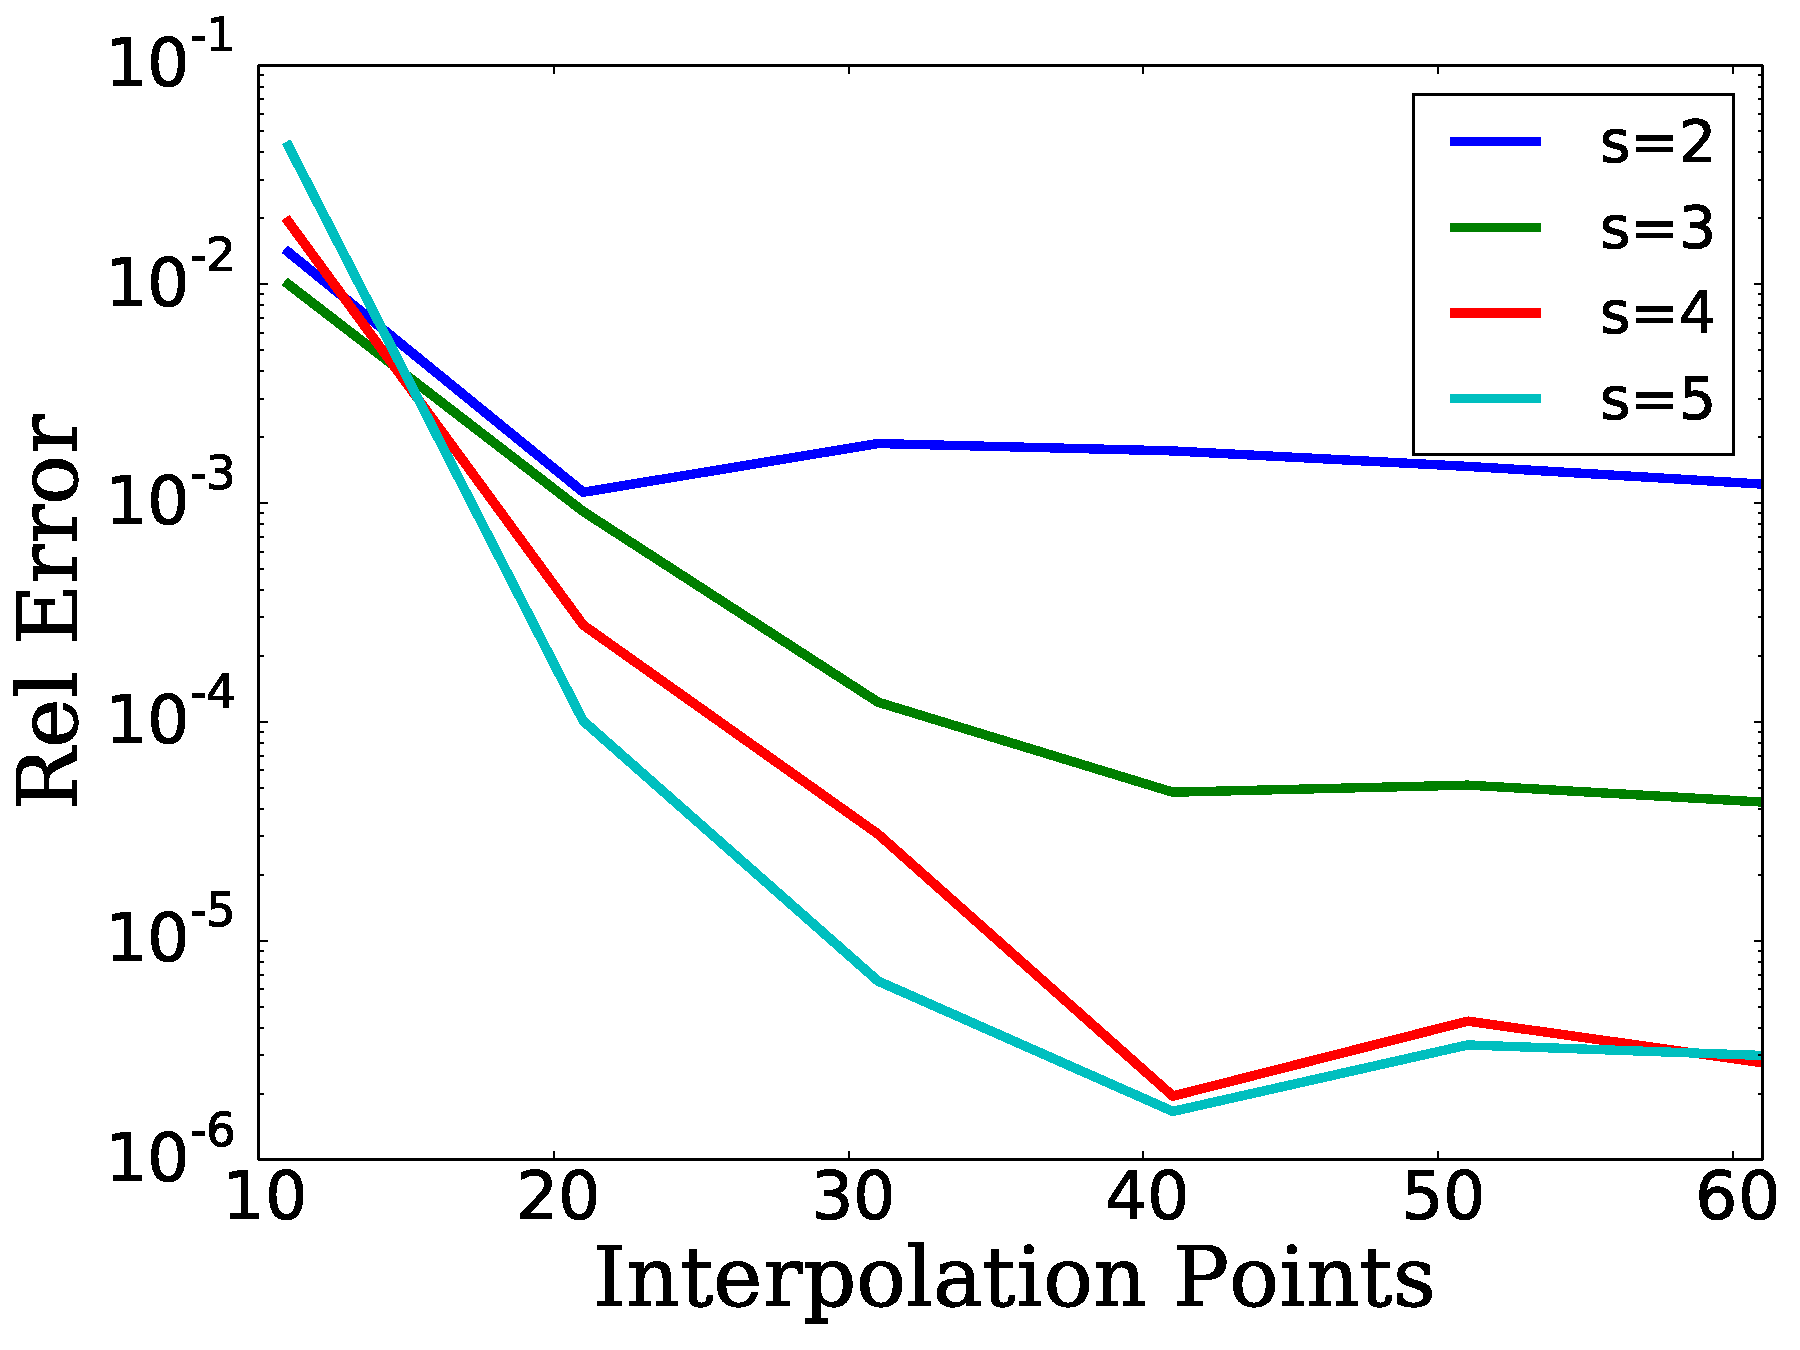
\includegraphics[width=\textwidth]{plots/msn_birkhoff_1d_single.pdf}
    \caption{Single Precision}
    \end{subfigure}
    \begin{subfigure}{0.45\textwidth}
    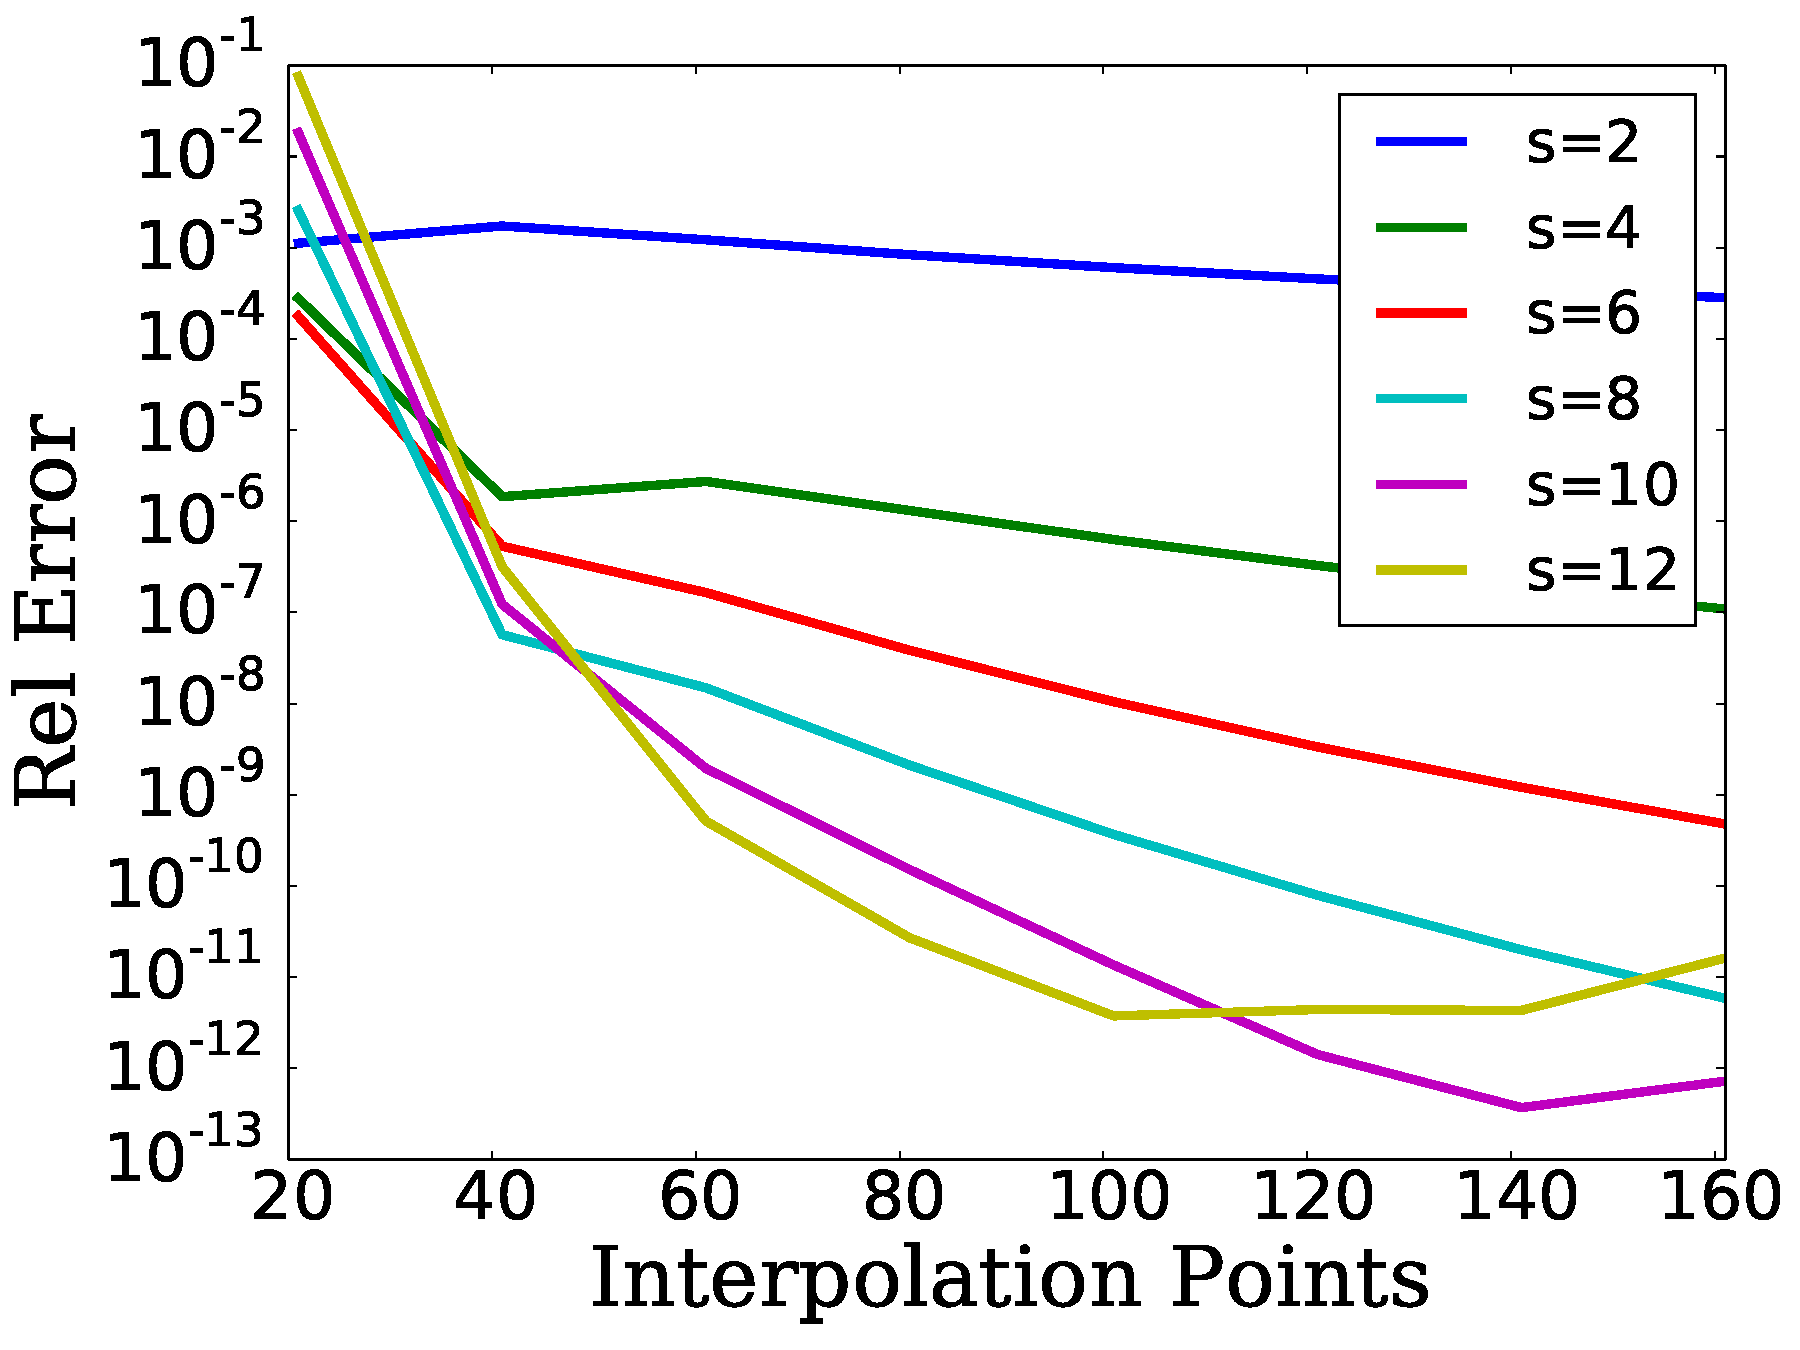
\includegraphics[width=\textwidth]{plots/msn_birkhoff_1d_double.pdf}
    \caption{Double Precision}
    \end{subfigure}
\caption[MSN 1D Birkhoff Interpolation Relative Error]{
Relative error results for MSN birkhoff interpolation on equally-spaced points
using both function and derivative values on the function $h(x)$
from Eq.~\eqref{eq:intro_runge_functions}
for various $s$ values using single and double precision.}
\label{fig:intro_msn_birkhoff_1d}
\end{figure}

\begin{figure}
\centering
    \begin{subfigure}{0.45\textwidth}
    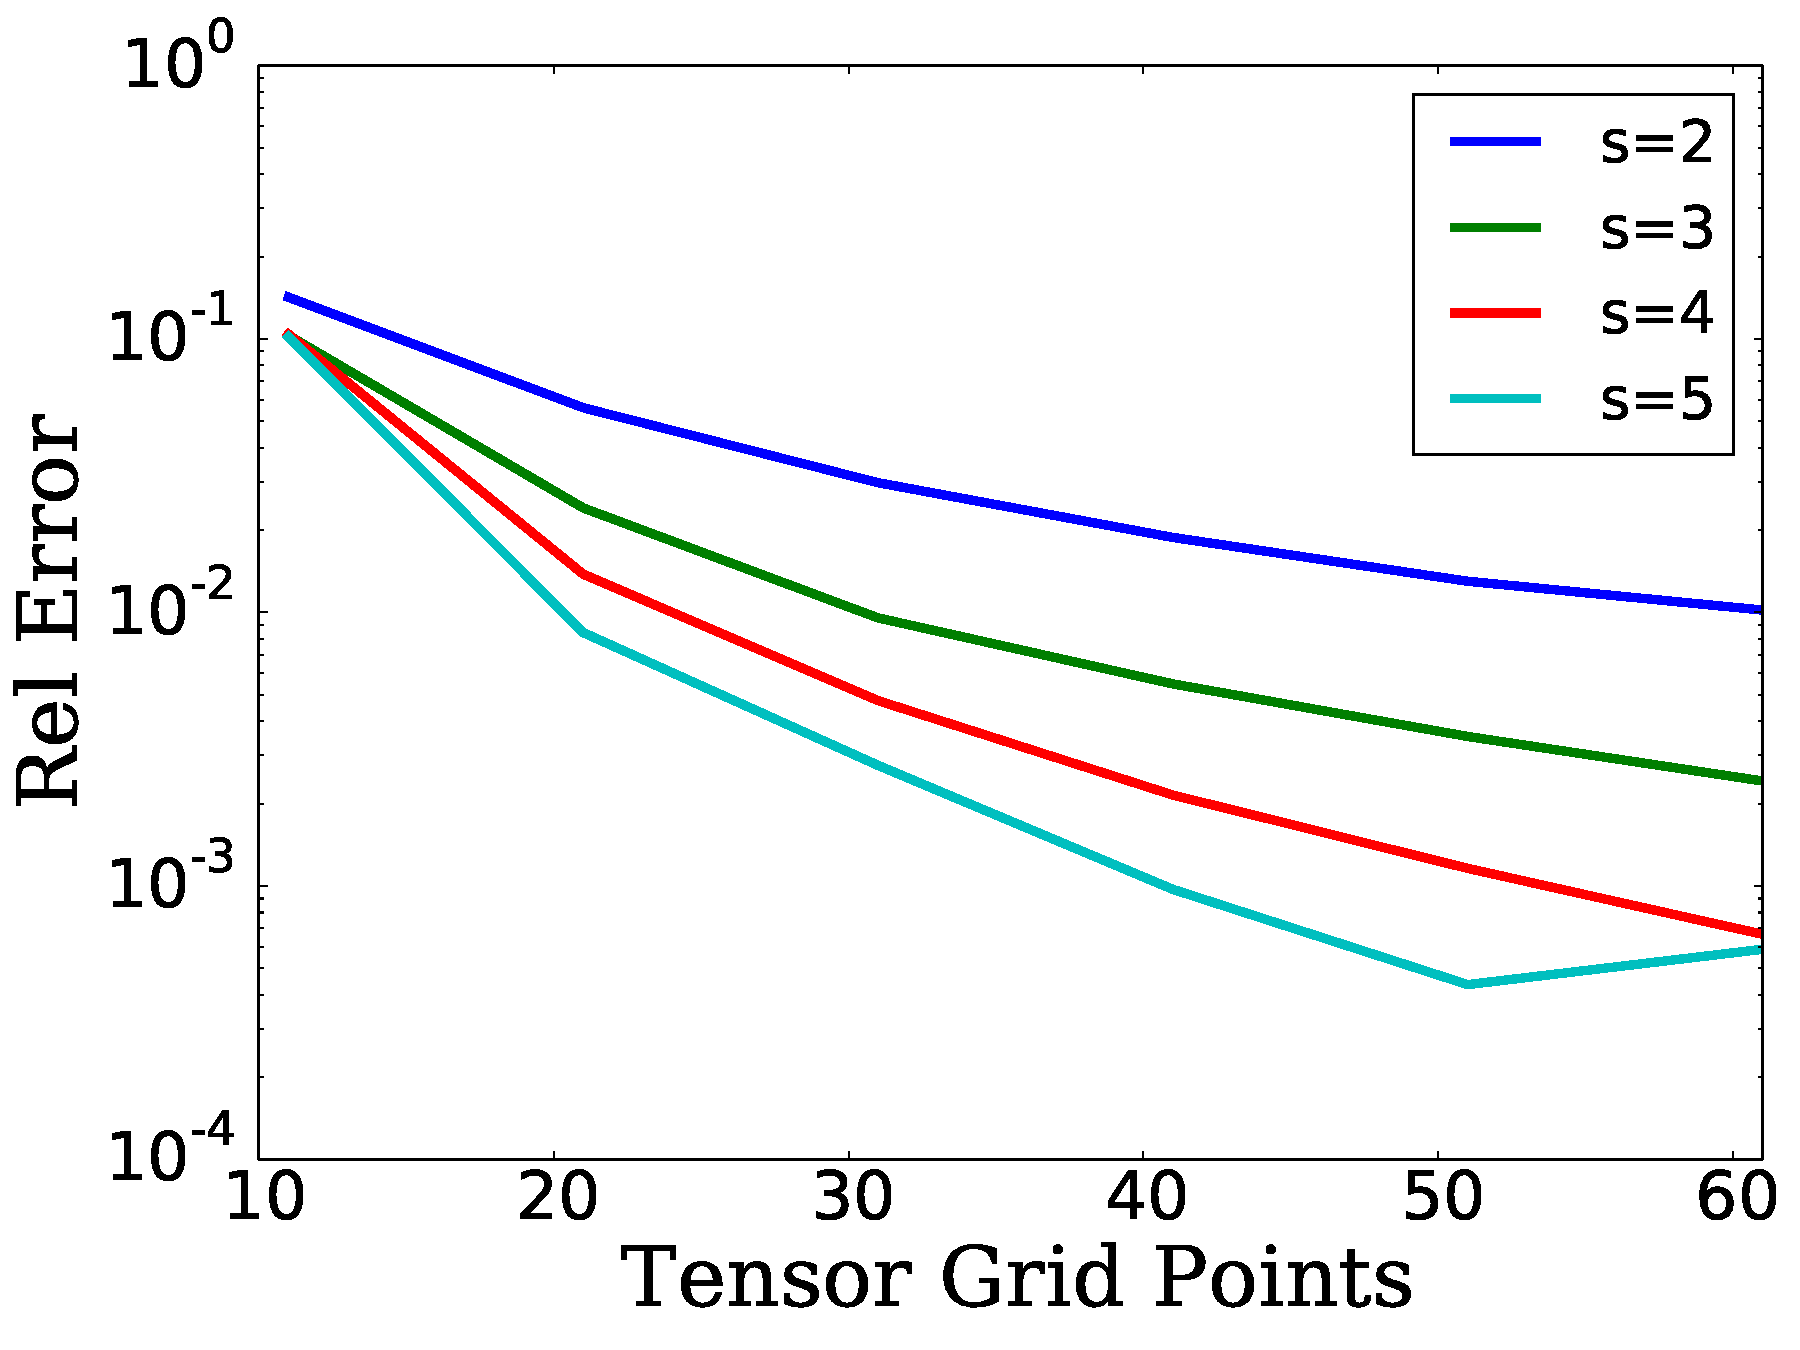
\includegraphics[width=\textwidth]{plots/msn_birkhoff_2d_single.pdf}
    \caption{Single Precision}
    \end{subfigure}
    \begin{subfigure}{0.45\textwidth}
    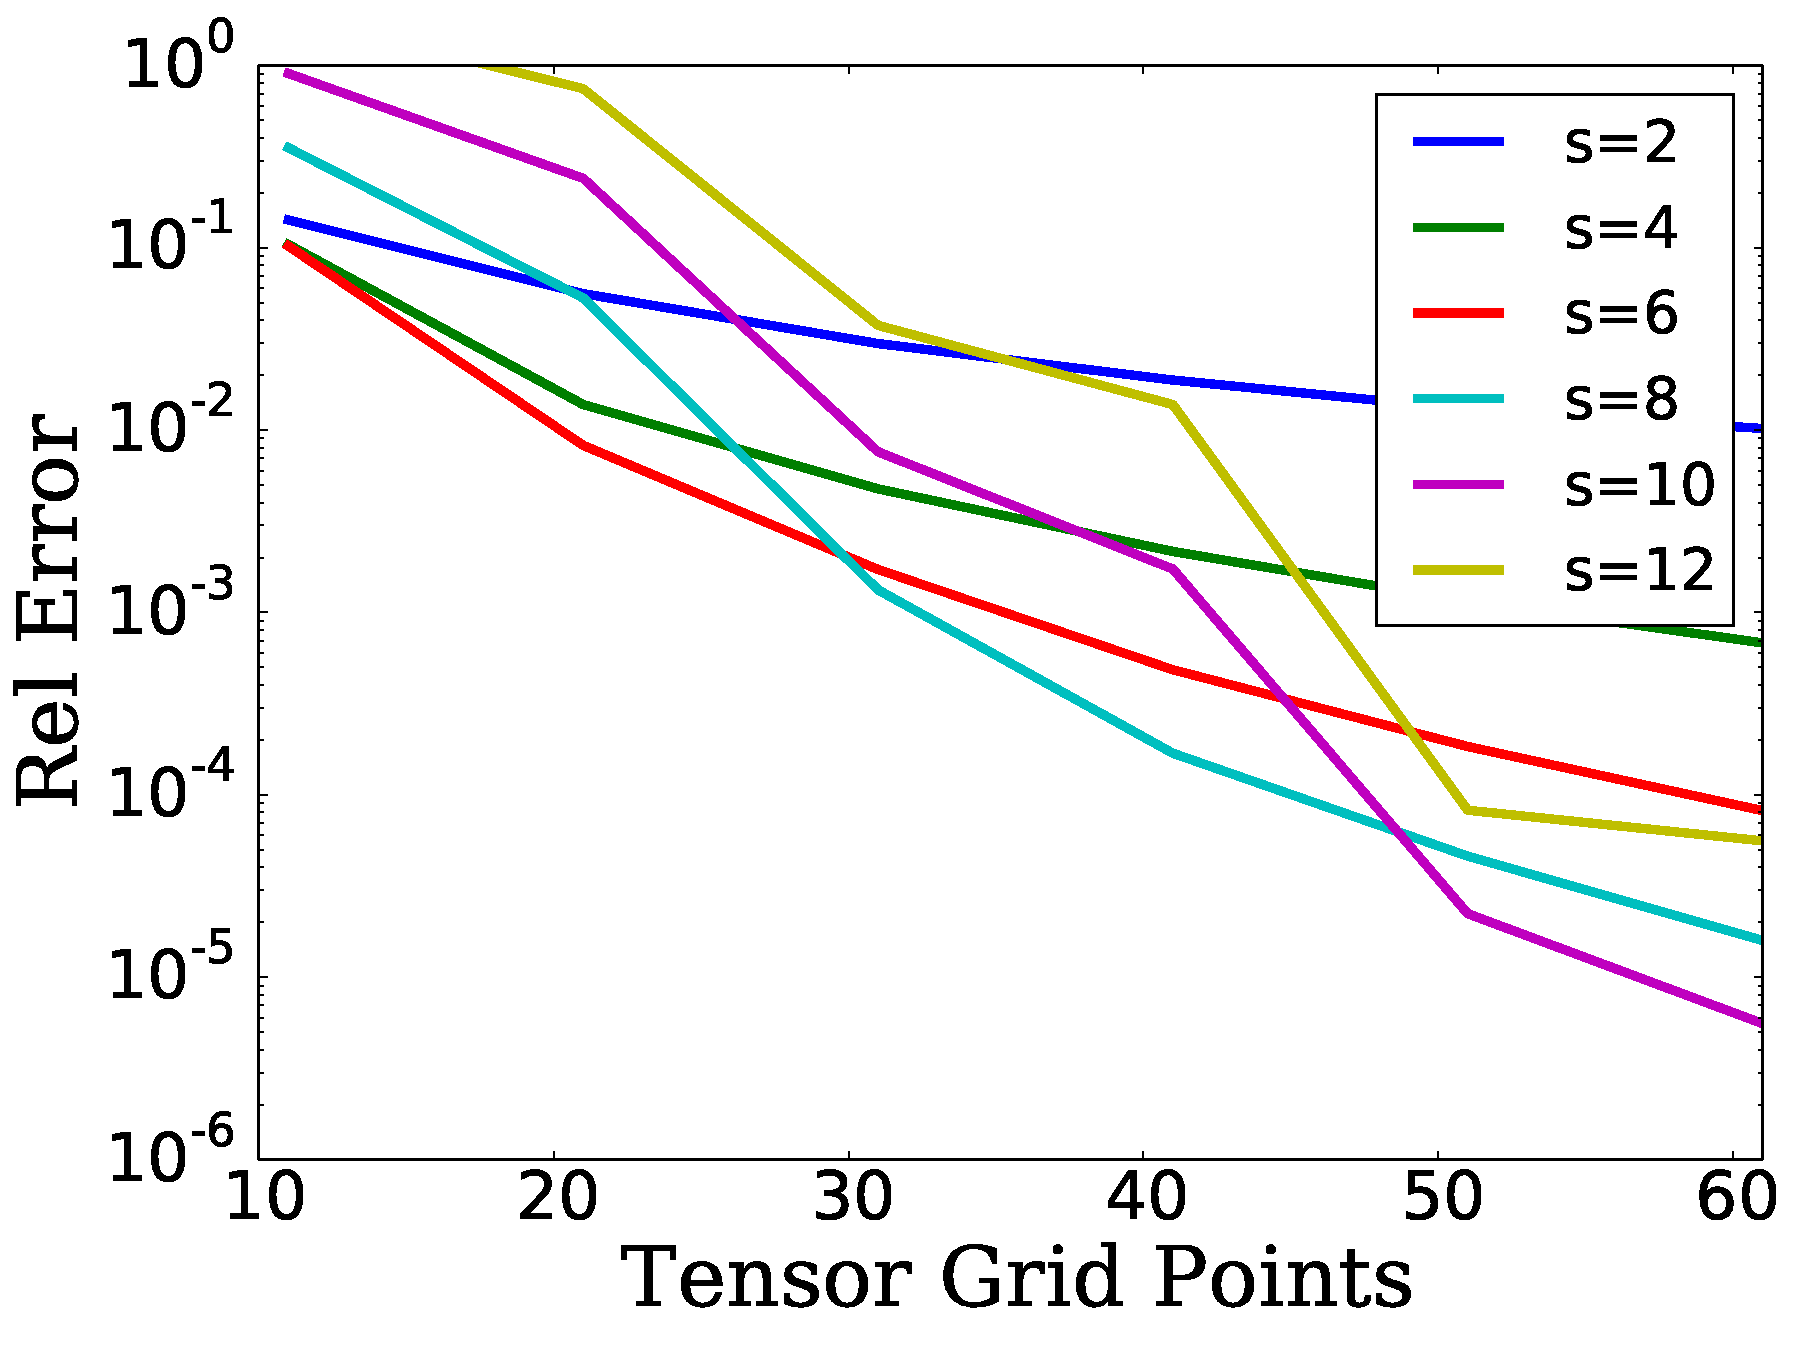
\includegraphics[width=\textwidth]{plots/msn_birkhoff_2d_double.pdf}
    \caption{Double Precision}
    \end{subfigure}
\caption[MSN 2D Birkhoff Interpolation Relative Error]{
Relative error results for MSN birkhoff interpolation on equally-spaced
tensor-grid points using both function and derivative values
on the function $g(x)$ from Eq.~\eqref{eq:intro_runge_functions}
for various $s$ values using single and double precision.}
\label{fig:intro_msn_birkhoff_2d}
\end{figure}







\section{Dissertation Outline}
\label{sec:dis_outline}

As we noted above, the slow methods for solving problems using
MSN become difficult in 2D and practically impossible in 3D
due to memory requirements and flop count. With the eventual
desire to use MSN to solve 3D PDEs,
we will need to take advantage of \emph{everything} we can.
Keeping this in mind, the focus of this dissertation
will be developing fast algorithms for solving interpolation
and differential equations using the MSN method on Chebyshev nodes
and express our solution in a Chebyshev polynomial basis.
We review notation conventions and structured
matrices in Chapter~\ref{chap:K_and_R}.
In Chapter~\ref{chap:CV_Prop}, we review some of the properties
of Chebyshev-Vandermonde matrices which arise when developing
these fast algorithms.
Matrix factorizations important for interpolation problems are
discussed in Chapters~\ref{chap:CV_mat_1D_I} and \ref{chap:CV_mat_HD_I}.
Using these factorizations, we present examples of MSN approximation
in Chapter~\ref{chap:func_interp}.
Next, we present new proofs showing that our fast methods
will converge to the solution under minimal smoothness assumptions
of the underlying function in Chapter~\ref{chap:cvip_converge}.
We investigate fast algorithms for Boundary Value Problems for ODEs
in Chapter~\ref{chap:fast_ode}.

In the Chapter~\ref{chap:random}, we discuss results related
to randomized low-rank approximations, unrelated to the previous work.
Some of this was discussed in~\cite{randomHSSLBL}
but more details and examples will be shown here.



\section{Algorithms Similar to the MSN Method}
\label{sec:similar_methods}

The ideas pursued in this dissertation are similar to those
used by Chebfun~\cite{driscoll2014chebfun}, a software package
in \textsc{Matlab}~\cite{guide1998mathworks} which attempts
to have the ``feel'' of symbolic software with the speed
of numerics.
The book Approximation Theory and Approximation Practice~\cite{ATAP}
uses Chebfun to introduce the field of  Approximation Theory.
Here, we focus on investigating fast algorithms based
on values computed on Chebyshev polynomial roots.
This is similar to the fast algorithms present in Chebfun,
which computes values on the Chebyshev polynomial extrema.
The book Exploring ODEs~\cite{ExpODEs} also uses
Chebfun to introduce advanced differential equation topics.
The methods in~\cite{ExpODEs} are built on the work
from~\cite{driscoll2015rectangular,aurentz2017block,xu2015explicit}
and are incorporated into Chebfun.
Although spectral methods are well-known~\cite{boyd2001chebyshev},
\cite{aurentz2017block} \emph{adds} additional rows
to the square linear system to impose boundary or other requirements
instead of replacing rows.
Naturally, this requires increasing the degree of the approximation.
The work presented here does not force a square system, which allows
us to add a finite number of additional requirements which do not
affect the asymptotic complexity of the overall algorithm.
From~\cite[Appendix A]{ExpODEs}, it appears that Chebfun uses
standard dense linear algebra algorithms to solve its ODEs.
This is unfortunate, because the linear systems arising from ODEs
are highly structured when approximated on Chebyshev nodes.
This dissertation will show this structure and construct associated
fast algorithms.
The work here could be used to speedup the Chebfun ODE solver.
